% This is "sig-alternate.tex" V1.9 April 2009
% This file should be compiled with V2.4 of "sig-alternate.cls" April 2009
%
% This example file demonstrates the use of the 'sig-alternate.cls'
% V2.4 LaTeX2e document class file. It is for those submitting
% articles to ACM Conference Proceedings WHO DO NOT WISH TO
% STRICTLY ADHERE TO THE SIGS (PUBS-BOARD-ENDORSED) STYLE.
% The 'sig-alternate.cls' file will produce a similar-looking,
% albeit, 'tighter' paper resulting in, invariably, fewer pages.
%
% ----------------------------------------------------------------------------------------------------------------
% This .tex file (and associated .cls V2.4) produces:
%       1) The Permission Statement
%       2) The Conference (location) Info information
%       3) The Copyright Line with ACM data
%       4) NO page numbers
%
% as against the acm_proc_article-sp.cls file which
% DOES NOT produce 1) thru' 3) above.
%
% Using 'sig-alternate.cls' you have control, however, from within
% the source .tex file, over both the CopyrightYear
% (defaulted to 200X) and the ACM Copyright Data
% (defaulted to X-XXXXX-XX-X/XX/XX).
% e.g.
% \CopyrightYear{2007} will cause 2007 to appear in the copyright line.
% \crdata{0-12345-67-8/90/12} will cause 0-12345-67-8/90/12 to appear in the copyright line.
%
% ---------------------------------------------------------------------------------------------------------------
% This .tex source is an example which *does* use
% the .bib file (from which the .bbl file % is produced).
% REMEMBER HOWEVER: After having produced the .bbl file,
% and prior to final submission, you *NEED* to 'insert'
% your .bbl file into your source .tex file so as to provide
% ONE 'self-contained' source file.
%
% ================= IF YOU HAVE QUESTIONS =======================
% Questions regarding the SIGS styles, SIGS policies and
% procedures, Conferences etc. should be sent to
% Adrienne Griscti (griscti@acm.org)
%
% Technical questions _only_ to
% Gerald Murray (murray@hq.acm.org)
% ===============================================================
%
% For tracking purposes - this is V1.9 - April 2009

\documentclass{Group6_Phase1}

\begin{document}
%
% --- Author Metadata here ---
%\conferenceinfo{WOODSTOCK}{'97 El Paso, Texas USA}
%\CopyrightYear{2007} % Allows default copyright year (20XX) to be over-ridden - IF NEED BE.
%\crdata{0-12345-67-8/90/01}  % Allows default copyright data (0-89791-88-6/97/05) to be over-ridden - IF NEED BE.
% --- End of Author Metadata ---

\title{Group 6 - Phase 1}
%\subtitle{[Extended Abstract]}
%
% You need the command \numberofauthors to handle the 'placement
% and alignment' of the authors beneath the title.
%
% For aesthetic reasons, we recommend 'three authors at a time'
% i.e. three 'name/affiliation blocks' be placed beneath the title.
%
% NOTE: You are NOT restricted in how many 'rows' of
% "name/affiliations" may appear. We just ask that you restrict
% the number of 'columns' to three.
%
% Because of the available 'opening page real-estate'
% we ask you to refrain from putting more than six authors
% (two rows with three columns) beneath the article title.
% More than six makes the first-page appear very cluttered indeed.
%
% Use the \alignauthor commands to handle the names
% and affiliations for an 'aesthetic maximum' of six authors.
% Add names, affiliations, addresses for
% the seventh etc. author(s) as the argument for the
% \additionalauthors command.
% These 'additional authors' will be output/set for you
% without further effort on your part as the last section in
% the body of your article BEFORE References or any Appendices.

\numberofauthors{2} %  in this sample file, there are a *total*
% of EIGHT authors. SIX appear on the 'first-page' (for formatting
% reasons) and the remaining two appear in the \additionalauthors section.
%
\author{
% You can go ahead and credit any number of authors here,
% e.g. one 'row of three' or two rows (consisting of one row of three
% and a second row of one, two or three).
%
% The command \alignauthor (no curly braces needed) should
% precede each author name, affiliation/snail-mail address and
% e-mail address. Additionally, tag each line of
% affiliation/address with \affaddr, and tag the
% e-mail address with \email.
%
%	1st. author
	\alignauthor
		Kevin Dombrosky\\
		       \affaddr{Rochester Institute of Technology Student}\\
		       \affaddr{610 Park Point Dr}\\
		       \affaddr{Rochester, New York 14623}\\
		       \email{kfd6490@rit.edu}
%	2nd. author
	\alignauthor
		Brittany Purcell\\
		       \affaddr{Rochester Institute of Technology Student}\\
		       \affaddr{107 Weldon Street}\\
		       \affaddr{Rochester, New York 14611}\\
		       \email{blp6903@rit.edu}
}

\maketitle
\begin{abstract}
This paper discusses the progression of the group project for Group 6 in the Intro to Big Data class at Rochester Institute of Technology, CSCI-620. The paper will further explain the work that has been done so far, what will be done in the future, and what the expectations are for the finished project. 
\end{abstract}

\keywords{Phase 1, Group 6, Plants}

\section{Introduction}
The group project for CSCI-620, Intro to Big Data at Rochester Institute of Technology has been underway for 7 weeks now. Is has been about a month since the initial submission of Phase-0 which laid out the data set and plan for the project.

Of the two requirements for the project, which include a database management system (DBMS), and having some form of database analytic, most of the work so far has been focused on the database analytic. During the last phase the dataset was chosen as well as a baseline for a visualization. As a reminder, Group 6 planned on creating an application that shows the geographical location of various types of plants in the United States and Canada using the Plants dataset from the UCI Machine Learning Repository. The database system is intended to be the relational database, MySQL. The analytics component is intended to be a visualization of what states and provinces have each plant within them.

There has been steady progression toward this goal, and so far there have been no changes to the visualization design, or the dataset. 
\\\\\\\\

\section{Body}

\subsection{Database}
As a reminder, the dataset will be set up in a MySQL database, and will be inserted using a script of some sort. The dataset being used is the Plants dataset from the UCI Machine Learning Repository (http://archive.ics.uci.edu/ml \\* /datasets/Plants). The information found in the database consists of a plant and its location in the United States/Canada. Below is the Entity-relationship(ER) diagram which was developed by Group 6. This diagram is the basis for how the information from the dataset will be stored in the database. 

\begin{figure}[htb]
	\centering
	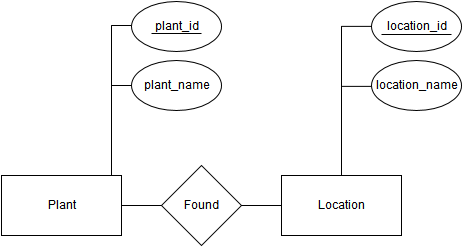
\includegraphics[scale=0.5]{FinalProject_ERdiagram.png}
	\caption{The ER diagram which represents the organization of the data in the database.}
\end{figure}

This is how the information will be stored within the database, and later when information needs to be accessed this will help making the proper calls to the database. There will be three tables within the database. The first, holding the information on the plants. This will consist of an ID for the plants, as well as the name of the plant associated with the ID. The locations will be very similar. The location chart will have a location ID, as well as the name of the location. Lastly, there will be a chart which compares the two items. This chart will map a plant-id to a location-id. That way, when a user is searching through the visualization the database will know what plants are in which location. 


\subsection{Application}
Group 6 decided to create a visualization for this class, which was discussed in Phase-0. As a recap, the visualization will consist of a map(functional for only the United States and Canada), as well as a search box for the user to search for a certain plant. This has been created, and the screen shot of the application is in Figure 2 below. 

This application is a web page that will be written in Jade Markup Language with CSS. This is the language that is most familiar to the group, after one of the members worked with the language all summer on an independent project. The basic blueprint for the web page has already been created(again, see Figure 2), but it has not yet been hooked up to the database. 

Ultimately, there will be (on the left hand side of the website right below the search bar) a list of plants that are found in the database. The user can search for a specific plant (using the search bar) which will highlight the regions that plant is located. Otherwise, the user can choose a plant from the list, and it will do the same thing. Another option for users would be to select a region they are interested in, and the list on the left would change to be only plants that can be found in that area. 

\begin{figure}[htb]
	\centering
	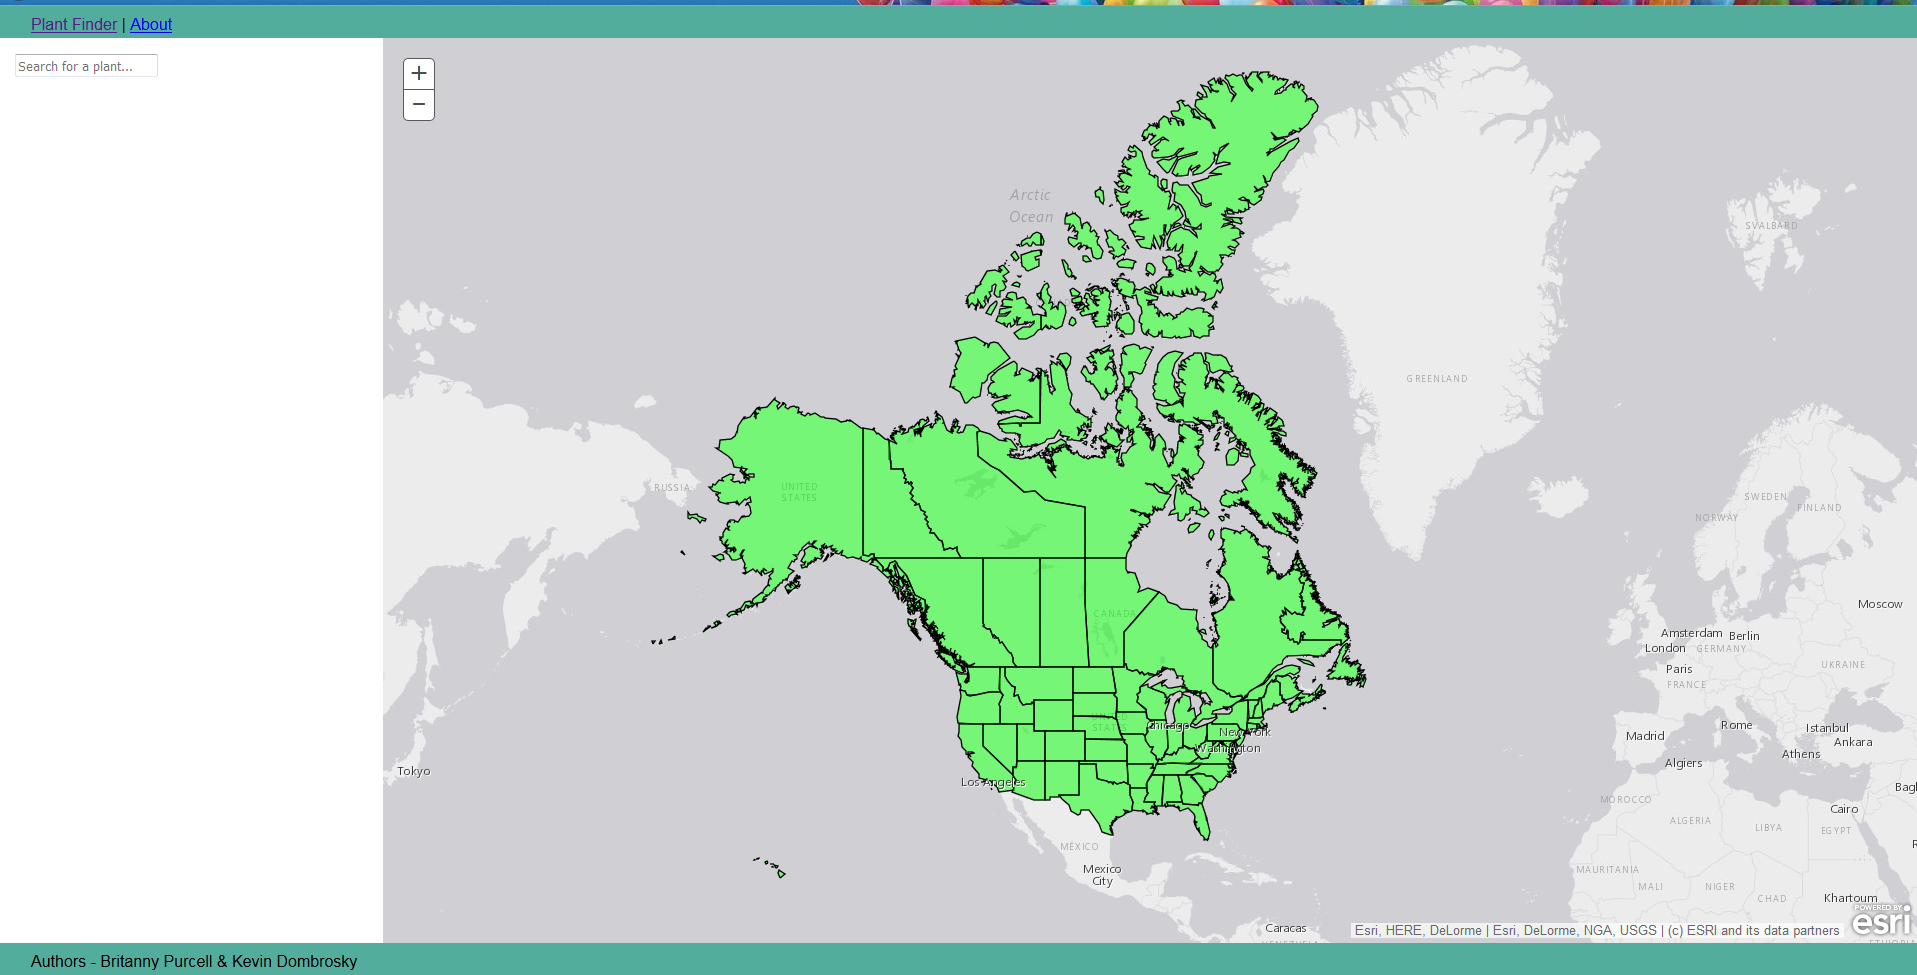
\includegraphics[scale=0.17]{Website_Screenshot.png}
	\caption{A screen shot of the website being used for the application.}
\end{figure}
\subsection{Communication}
In order for the website and database to communicate, the database will be setup on a Node.js server. This will allow the website to request information from the database in order for the user interface(UI) to change based on users requests. This is how the information will be transmitted from the database to the website. 

\subsection{Resources}
There are many different resources being used in order to develop the project. These include certain files, softwares, and online databases all assisting in the creation of the website and database. As it was already covered, the database is being set up as a MySQL database, the application will be a website visualization that is coded using Jade and CSS, and the database and website will communicate with a Node.js server. 

The code is being stored using GitHub, and is shared among all members of the group. This is a repository to store, download, and change the existing code. The code is being written in different platforms, some members are using Notepad++ to do the coding, while others are using Visual Studio Code. Once the code is written in each of these mediums, the code is added to the GitHub repository. 

LaTeX is being used to write the ACM style templates, which is the document you are currently reading, and Visual Studio Code is used for the README(which will walk users through how to run the program and access the website).

The README will be provided to establish step-by-step instructions on downloading and installing necessary software, and (once the software is installed), how to run the project and access the website. 


\section{Conclusions}
The group has already made some progress towards finishing the project. This includes work on both the application as well as the database. There is still much work that needs to be done, but most of the thinking and setting up has been finished. Languages and applications have been chosen and are in the process of being set up. Below is a quick list of what was done, what needs to be done, and deliverables that have been set.  

\begin{description}
	\item[Accomplished:] \hfill
	\begin{itemize}
		\item Developed ER Diagram
		\item Created Website Wire Frame
		\item Setup Website
		\item Conceptualized Application Utilization
	\end{itemize}
	
	\item[To Be Done:] \hfill
	\begin{itemize}
		\item Write Python Script for Database Input
		\item Set Up Database
		\item Establish Communication Between Website and Database
		\item Display Information on Website
		\item Change Display based on User Input
	\end{itemize}
	
	\item[Resources] \hfill
	\begin{itemize}
		\item GitHub
		\item LaTeX
		\item Node.js
		\item Notepad++
		\item Visual Studio Code
	\end{itemize}
	
	\item[Files] \hfill
	\begin{itemize}
		\item README
		\item Group6-Phase1
		\item CSCI620-master (Folder)
	\end{itemize}
\end{description}


\end{document}  % This is where a 'short' article might terminate
